%% bare_jrnl.tex
%% V1.3
%% 2007/01/11
%% by Michael Shell
%% see http://www.michaelshell.org/
%% for current contact information.
%%
%% This is a skeleton file demonstrating the use of IEEEtran.cls
%% (requires IEEEtran.cls version 1.7 or later) with an IEEE journal paper.
%%
%% Support sites:
%% http://www.michaelshell.org/tex/ieeetran/
%% http://www.ctan.org/tex-archive/macros/latex/contrib/IEEEtran/
%% and
%% http://www.ieee.org/

% *** Authors should verify (and, if needed, correct) their LaTeX system  ***
% *** with the testflow diagnostic prior to trusting their LaTeX platform ***
% *** with production work. IEEE's font choices can trigger bugs that do  ***
% *** not appear when using other class files.                            ***
% The testflow support page is at:
% http://www.michaelshell.org/tex/testflow/

%%*************************************************************************
%% Legal Notice:
%% This code is offered as-is without any warranty either expressed or
%% implied; without even the implied warranty of MERCHANTABILITY or
%% FITNESS FOR A PARTICULAR PURPOSE! 
%% User assumes all risk.
%% In no event shall IEEE or any contributor to this code be liable for
%% any damages or losses, including, but not limited to, incidental,
%% consequential, or any other damages, resulting from the use or misuse
%% of any information contained here.
%%
%% All comments are the opinions of their respective authors and are not
%% necessarily endorsed by the IEEE.
%%
%% This work is distributed under the LaTeX Project Public License (LPPL)
%% ( http://www.latex-project.org/ ) version 1.3, and may be freely used,
%% distributed and modified. A copy of the LPPL, version 1.3, is included
%% in the base LaTeX documentation of all distributions of LaTeX released
%% 2003/12/01 or later.
%% Retain all contribution notices and credits.
%% ** Modified files should be clearly indicated as such, including  **
%% ** renaming them and changing author support contact information. **
%%
%% File list of work: IEEEtran.cls, IEEEtran_HOWTO.pdf, bare_adv.tex,
%%                    bare_conf.tex, bare_jrnl.tex, bare_jrnl_compsoc.tex
%%*************************************************************************

% Note that the a4paper option is mainly intended so that authors in
% countries using A4 can easily print to A4 and see how their papers will
% look in print - the typesetting of the document will not typically be
% affected with changes in paper size (but the bottom and side margins will).
% Use the testflow package mentioned above to verify correct handling of
% both paper sizes by the user's LaTeX system.
%
% Also note that the "draftcls" or "draftclsnofoot", not "draft", option
% should be used if it is desired that the figures are to be displayed in
% draft mode.
%
\documentclass[journal]{IEEEtran}

%
% If IEEEtran.cls has not been installed into the LaTeX system files,
% manually specify the path to it like:
% \documentclass[journal]{../sty/IEEEtran}

% Some very useful LaTeX packages include:
% (uncomment the ones you want to load)

% *** MISC UTILITY PACKAGES ***
%
%\usepackage{ifpdf}
% Heiko Oberdiek's ifpdf.sty is very useful if you need conditional
% compilation based on whether the output is pdf or dvi.
% usage:
% \ifpdf
%   % pdf code
% \else
%   % dvi code
% \fi
% The latest version of ifpdf.sty can be obtained from:
% http://www.ctan.org/tex-archive/macros/latex/contrib/oberdiek/
% Also, note that IEEEtran.cls V1.7 and later provides a builtin
% \ifCLASSINFOpdf conditional that works the same way.
% When switching from latex to pdflatex and vice-versa, the compiler may
% have to be run twice to clear warning/error messages.

% *** CITATION PACKAGES ***
%
%\usepackage{cite}
% cite.sty was written by Donald Arseneau
% V1.6 and later of IEEEtran pre-defines the format of the cite.sty package
% \cite{} output to follow that of IEEE. Loading the cite package will
% result in citation numbers being automatically sorted and properly
% "compressed/ranged". e.g., [1], [9], [2], [7], [5], [6] without using
% cite.sty will become [1], [2], [5]--[7], [9] using cite.sty. cite.sty's
% \cite will automatically add leading space, if needed. Use cite.sty's
% noadjust option (cite.sty V3.8 and later) if you want to turn this off.
% cite.sty is already installed on most LaTeX systems. Be sure and use
% version 4.0 (2003-05-27) and later if using hyperref.sty. cite.sty does
% not currently provide for hyperlinked citations.
% The latest version can be obtained at:
% http://www.ctan.org/tex-archive/macros/latex/contrib/cite/
% The documentation is contained in the cite.sty file itself.

% *** GRAPHICS RELATED PACKAGES ***
%
\usepackage{graphicx}
\usepackage{epstopdf}
%\ifCLASSINFOpdf
%\usepackage[pdftex]{graphicx}
  % declare the path(s) where your graphic files are
%\graphicspath{{../pdf/}{../jpeg/}{../eps}}
  % and their extensions so you won't have to specify these with
  % every instance of \includegraphics
%\DeclareGraphicsExtensions{.pdf,.jpeg,.png,.eps}
%\else
  % or other class option (dvipsone, dvipdf, if not using dvips). graphicx
  % will default to the driver specified in the system graphics.cfg if no
  % driver is specified.
%\usepackage[dvips]{graphicx}
  % declare the path(s) where your graphic files are
%\graphicspath{{../eps/}}
  % and their extensions so you won't have to specify these with
  % every instance of \includegraphics
%\DeclareGraphicsExtensions{.eps}
%\fi
% graphicx was written by David Carlisle and Sebastian Rahtz. It is
% required if you want graphics, photos, etc. graphicx.sty is already
% installed on most LaTeX systems. The latest version and documentation can
% be obtained at: 
% http://www.ctan.org/tex-archive/macros/latex/required/graphics/
% Another good source of documentation is "Using Imported Graphics in
% LaTeX2e" by Keith Reckdahl which can be found as epslatex.ps or
% epslatex.pdf at: http://www.ctan.org/tex-archive/info/
%
% latex, and pdflatex in dvi mode, support graphics in encapsulated
% postscript (.eps) format. pdflatex in pdf mode supports graphics
% in .pdf, .jpeg, .png and .mps (metapost) formats. Users should ensure
% that all non-photo figures use a vector format (.eps, .pdf, .mps) and
% not a bitmapped formats (.jpeg, .png). IEEE frowns on bitmapped formats
% which can result in "jaggedy"/blurry rendering of lines and letters as
% well as large increases in file sizes.
%
% You can find documentation about the pdfTeX application at:
% http://www.tug.org/applications/pdftex

% *** MATH PACKAGES ***
%
\usepackage[cmex10]{amsmath}
% A popular package from the American Mathematical Society that provides
% many useful and powerful commands for dealing with mathematics. If using
% it, be sure to load this package with the cmex10 option to ensure that
% only type 1 fonts will utilized at all point sizes. Without this option,
% it is possible that some math symbols, particularly those within
% footnotes, will be rendered in bitmap form which will result in a
% document that can not be IEEE Xplore compliant!
%
% Also, note that the amsmath package sets \interdisplaylinepenalty to 10000
% thus preventing page breaks from occurring within multiline equations. Use:
%\interdisplaylinepenalty=2500
% after loading amsmath to restore such page breaks as IEEEtran.cls normally
% does. amsmath.sty is already installed on most LaTeX systems. The latest
% version and documentation can be obtained at:
% http://www.ctan.org/tex-archive/macros/latex/required/amslatex/math/

% *** SPECIALIZED LIST PACKAGES ***
%
%\usepackage{algorithmic}
% algorithmic.sty was written by Peter Williams and Rogerio Brito.
% This package provides an algorithmic environment fo describing algorithms.
% You can use the algorithmic environment in-text or within a figure
% environment to provide for a floating algorithm. Do NOT use the algorithm
% floating environment provided by algorithm.sty (by the same authors) or
% algorithm2e.sty (by Christophe Fiorio) as IEEE does not use dedicated
% algorithm float types and packages that provide these will not provide
% correct IEEE style captions. The latest version and documentation of
% algorithmic.sty can be obtained at:
% http://www.ctan.org/tex-archive/macros/latex/contrib/algorithms/
% There is also a support site at:
% http://algorithms.berlios.de/index.html
% Also of interest may be the (relatively newer and more customizable)
% algorithmicx.sty package by Szasz Janos:
% http://www.ctan.org/tex-archive/macros/latex/contrib/algorithmicx/

% *** ALIGNMENT PACKAGES ***
%
\usepackage{array}
% Frank Mittelbach's and David Carlisle's array.sty patches and improves
% the standard LaTeX2e array and tabular environments to provide better
% appearance and additional user controls. As the default LaTeX2e table
% generation code is lacking to the point of almost being broken with
% respect to the quality of the end results, all users are strongly
% advised to use an enhanced (at the very least that provided by array.sty)
% set of table tools. array.sty is already installed on most systems. The
% latest version and documentation can be obtained at:
% http://www.ctan.org/tex-archive/macros/latex/required/tools/

\usepackage{mdwmath}
\usepackage{mdwtab}
% Also highly recommended is Mark Wooding's extremely powerful MDW tools,
% especially mdwmath.sty and mdwtab.sty which are used to format equations
% and tables, respectively. The MDWtools set is already installed on most
% LaTeX systems. The lastest version and documentation is available at:
% http://www.ctan.org/tex-archive/macros/latex/contrib/mdwtools/

% IEEEtran contains the IEEEeqnarray family of commands that can be used to
% generate multiline equations as well as matrices, tables, etc., of high
% quality.

\usepackage{eqparbox}
% Also of notable interest is Scott Pakin's eqparbox package for creating
% (automatically sized) equal width boxes - aka "natural width parboxes".
% Available at:
% http://www.ctan.org/tex-archive/macros/latex/contrib/eqparbox/

% *** SUBFIGURE PACKAGES ***
%\usepackage[tight,footnotesize]{subfigure}
% subfigure.sty was written by Steven Douglas Cochran. This package makes it
% easy to put subfigures in your figures. e.g., "Figure 1a and 1b". For IEEE
% work, it is a good idea to load it with the tight package option to reduce
% the amount of white space around the subfigures. subfigure.sty is already
% installed on most LaTeX systems. The latest version and documentation can
% be obtained at:
% http://www.ctan.org/tex-archive/obsolete/macros/latex/contrib/subfigure/
% subfigure.sty has been superceeded by subfig.sty.

%\usepackage[caption=false]{caption}
%\usepackage[font=footnotesize]{subfig}
% subfig.sty, also written by Steven Douglas Cochran, is the modern
% replacement for subfigure.sty. However, subfig.sty requires and
% automatically loads Axel Sommerfeldt's caption.sty which will override
% IEEEtran.cls handling of captions and this will result in nonIEEE style
% figure/table captions. To prevent this problem, be sure and preload
% caption.sty with its "caption=false" package option. This is will preserve
% IEEEtran.cls handing of captions. Version 1.3 (2005/06/28) and later 
% (recommended due to many improvements over 1.2) of subfig.sty supports
% the caption=false option directly:
%\usepackage[caption=false,font=footnotesize]{subfig}
%
% The latest version and documentation can be obtained at:
% http://www.ctan.org/tex-archive/macros/latex/contrib/subfig/
% The latest version and documentation of caption.sty can be obtained at:
% http://www.ctan.org/tex-archive/macros/latex/contrib/caption/

% *** FLOAT PACKAGES ***
%
%\usepackage{fixltx2e}
% fixltx2e, the successor to the earlier fix2col.sty, was written by
% Frank Mittelbach and David Carlisle. This package corrects a few problems
% in the LaTeX2e kernel, the most notable of which is that in current
% LaTeX2e releases, the ordering of single and double column floats is not
% guaranteed to be preserved. Thus, an unpatched LaTeX2e can allow a
% single column figure to be placed prior to an earlier double column
% figure. The latest version and documentation can be found at:
% http://www.ctan.org/tex-archive/macros/latex/base/

%\usepackage{stfloats}
% stfloats.sty was written by Sigitas Tolusis. This package gives LaTeX2e
% the ability to do double column floats at the bottom of the page as well
% as the top. (e.g., "\begin{figure*}[!b]" is not normally possible in
% LaTeX2e). It also provides a command:
%\fnbelowfloat
% to enable the placement of footnotes below bottom floats (the standard
% LaTeX2e kernel puts them above bottom floats). This is an invasive package
% which rewrites many portions of the LaTeX2e float routines. It may not work
% with other packages that modify the LaTeX2e float routines. The latest
% version and documentation can be obtained at:
% http://www.ctan.org/tex-archive/macros/latex/contrib/sttools/
% Documentation is contained in the stfloats.sty comments as well as in the
% presfull.pdf file. Do not use the stfloats baselinefloat ability as IEEE
% does not allow \baselineskip to stretch. Authors submitting work to the
% IEEE should note that IEEE rarely uses double column equations and
% that authors should try to avoid such use. Do not be tempted to use the
% cuted.sty or midfloat.sty packages (also by Sigitas Tolusis) as IEEE does
% not format its papers in such ways.

%\ifCLASSOPTIONcaptionsoff
%  \usepackage[nomarkers]{endfloat}
% \let\MYoriglatexcaption\caption
% \renewcommand{\caption}[2][\relax]{\MYoriglatexcaption[#2]{#2}}
%\fi
% endfloat.sty was written by James Darrell McCauley and Jeff Goldberg.
% This package may be useful when used in conjunction with IEEEtran.cls'
% captionsoff option. Some IEEE journals/societies require that submissions
% have lists of figures/tables at the end of the paper and that
% figures/tables without any captions are placed on a page by themselves at
% the end of the document. If needed, the draftcls IEEEtran class option or
% \CLASSINPUTbaselinestretch interface can be used to increase the line
% spacing as well. Be sure and use the nomarkers option of endfloat to
% prevent endfloat from "marking" where the figures would have been placed
% in the text. The two hack lines of code above are a slight modification of
% that suggested by in the endfloat docs (section 8.3.1) to ensure that
% the full captions always appear in the list of figures/tables - even if
% the user used the short optional argument of \caption[]{}.
% IEEE papers do not typically make use of \caption[]'s optional argument,
% so this should not be an issue. A similar trick can be used to disable
% captions of packages such as subfig.sty that lack options to turn off
% the subcaptions:
% For subfig.sty:
% \let\MYorigsubfloat\subfloat
% \renewcommand{\subfloat}[2][\relax]{\MYorigsubfloat[]{#2}}
% For subfigure.sty:
% \let\MYorigsubfigure\subfigure
% \renewcommand{\subfigure}[2][\relax]{\MYorigsubfigure[]{#2}}
% However, the above trick will not work if both optional arguments of
% the \subfloat/subfig command are used. Furthermore, there needs to be a
% description of each subfigure *somewhere* and endfloat does not add
% subfigure captions to its list of figures. Thus, the best approach is to
% avoid the use of subfigure captions (many IEEE journals avoid them anyway)
% and instead reference/explain all the subfigures within the main caption.
% The latest version of endfloat.sty and its documentation can obtained at:
% http://www.ctan.org/tex-archive/macros/latex/contrib/endfloat/
%
% The IEEEtran \ifCLASSOPTIONcaptionsoff conditional can also be used
% later in the document, say, to conditionally put the References on a 
% page by themselves.

% *** PDF, URL AND HYPERLINK PACKAGES ***
%
%\usepackage{url}
% url.sty was written by Donald Arseneau. It provides better support for
% handling and breaking URLs. url.sty is already installed on most LaTeX
% systems. The latest version can be obtained at:
% http://www.ctan.org/tex-archive/macros/latex/contrib/misc/
% Read the url.sty source comments for usage information. Basically,
% \url{my_url_here}.

% *** Do not adjust lengths that control margins, column widths, etc. ***
% *** Do not use packages that alter fonts (such as pslatex).         ***
% There should be no need to do such things with IEEEtran.cls V1.6 and later.
% (Unless specifically asked to do so by the journal or conference you plan
% to submit to, of course. )

% correct bad hyphenation here
\hyphenation{op-tical net-works semi-conduc-tor}

\begin{document}
%
% paper title
% can use linebreaks \\ within to get better formatting as desired
\title{Energy-based Particle Swarm Optimization: Collective Energy Homeostasis in Social Robots}
%
%
% author names and IEEE memberships
% note positions of commas and nonbreaking spaces ( ~ ) LaTeX will not break
% a structure at a ~ so this keeps an author's name from being broken across
% two lines.
% use \thanks{} to gain access to the first footnote area
% a separate \thanks must be used for each paragraph as LaTeX2e's \thanks
% was not built to handle multiple paragraphs
%

\author{Xin Zhou,
        Kai Xiao,
		Yongfeng Xia,
		Alei Liang,
		Haibing Guan*,
		Aboul Ella Hassanien% <-this % stops a space
%\thanks{M. Shell is with the Department
%of Electrical and Computer Engineering, Georgia Institute of Technology, Atlanta,
%GA, 30332 USA e-mail: (see http://www.michaelshell.org/contact.html).}% <-this % stops a space
%\thanks{J. Doe and J. Doe are with Anonymous University.}% <-this % stops a space
%\thanks{Manuscript received April 19, 2005; revised January 11, 2007.}}
\thanks{Xin Zhou, Xiao Kai, Yongfeng Xia, Alei Liang and Haibing Guan are with School of Software, Shanghai Key Laboratory of Scalable Computing and Systems, Shanghai Jiao Tong University, China, e-mail:\{zhouxin, youngsterxyf, liangalei, hbguan\}@sjtu.edu.cn, showkey@gmail.com}
\thanks{Aboul Ella Hassanien is with Information Technology Department, Faculty of Computer \& Information, Cairo University, Egypt, e-mail: Aboit-cairo@gmail.com}
}
% note the % following the last \IEEEmembership and also \thanks - 
% these prevent an unwanted space from occurring between the last author name
% and the end of the author line. i.e., if you had this:
% 
% \author{....lastname \thanks{...} \thanks{...} }
%                     ^------------^------------^----Do not want these spaces!
%
% a space would be appended to the last name and could cause every name on that
% line to be shifted left slightly. This is one of those "LaTeX things". For
% instance, "\textbf{A} \textbf{B}" will typeset as "A B" not "AB". To get
% "AB" then you have to do: "\textbf{A}\textbf{B}"
% \thanks is no different in this regard, so shield the last } of each \thanks
% that ends a line with a % and do not let a space in before the next \thanks.
% Spaces after \IEEEmembership other than the last one are OK (and needed) as
% you are supposed to have spaces between the names. For what it is worth,
% this is a minor point as most people would not even notice if the said evil
% space somehow managed to creep in.



% The paper headers
%%%%%%%%%%%%%%%%%%%%%%%%%%%%%%%%%%%%%%%%%%%%%%%%%%%%%%%
%\markboth{Journal of \LaTeX\ Class Files,~Vol.~6, No.~1, January~2007}%
%{Shell \MakeLowercase{\textit{et al.}}: Bare Demo of IEEEtran.cls for Journals}
% The only time the second header will appear is for the odd numbered pages
% after the title page when using the twoside option.
% 
% *** Note that you probably will NOT want to include the author's ***
% *** name in the headers of peer review papers.                   ***
% You can use \ifCLASSOPTIONpeerreview for conditional compilation here if
% you desire.

% If you want to put a publisher's ID mark on the page you can do it like
% this:
%\IEEEpubid{0000--0000/00\$00.00~\copyright~2007 IEEE}
% Remember, if you use this you must call \IEEEpubidadjcol in the second
% column for its text to clear the IEEEpubid mark.

% use for special paper notices
%\IEEEspecialpapernotice{(Invited Paper)}

% make the title area
\maketitle

\begin{abstract}
%\boldmath
Social robots, either appeared as single units or organized in groups, will be required to manage their own energy. Uneven energy distributed in a whole robotic group may cause the mission unable to be completed and deteriorate the system tolerance. Previous works have mainly focused on the energy exchanging method using battery charging system. This paper presents a novel approach for maintaining the energy homeostasis in social robots by improving Particle Swarm Optimization(PSO) algorithm to shift the tasks of a robot in the swarm. The proposed Energy-based PSO(EPSO) algorithm, by taking the currently available energy status and information in the vicinity into account, "exchanges" the energy of the robot indirectly by shifting tasks. Experimental results show that EPSO enbales social robots to maintain their energy homeostasis. Compared to the modified PSO in~\cite{Meng}, EPSO increases energy homeostasis performance by 48.7\% on variance. 
\end{abstract}
% IEEEtran.cls defaults to using nonbold math in the Abstract.
% This preserves the distinction between vectors and scalars. However,
% if the journal you are submitting to favors bold math in the abstract,
% then you can use LaTeX's standard command \boldmath at the very start
% of the abstract to achieve this. Many IEEE journals frown on math
% in the abstract anyway.

% Note that keywords are not normally used for peerreview papers.
\begin{IEEEkeywords}
Energy Homeostasis, Social Robots, Energy-based Particle Swarm Optimization.
\end{IEEEkeywords}

% For peer review papers, you can put extra information on the cover
% page as needed:
% \ifCLASSOPTIONpeerreview
% \begin{center} \bfseries EDICS Category: 3-BBND \end{center}
% \fi
%
% For peerreview papers, this IEEEtran command inserts a page break and
% creates the second title. It will be ignored for other modes.
\IEEEpeerreviewmaketitle

\section{Introduction}
\label{sec:1}
% The very first letter is a 2 line initial drop letter followed
% by the rest of the first word in caps.
% 
% form to use if the first word consists of a single letter:
% \IEEEPARstart{A}{demo} file is ....
% 
% form to use if you need the single drop letter followed by
% normal text (unknown if ever used by IEEE):
% \IEEEPARstart{A}{}demo file is ....
% 
% Some journals put the first two words in caps:
% \IEEEPARstart{T}{his demo} file is ....
% 
% Here we have the typical use of a "T" for an initial drop letter
% and "HIS" in caps to complete the first word.
\IEEEPARstart{S}{ocial} robots are robots that operate in swarm where individuals are capable of mutually sharing food(energy), task, information, recongnition and even intelligence~\cite{Ngo}. A robot in a swarm will get inactive when its energy is depleted, and the whole swarm will not work if a certain number of robots in the swarm stop. Thus, the social robots have to manage their energy in an intelligence manner in order to complete their mission. To make the system energy autonomously manageable, the robot has to fulfill the criteria of self-sufficiency~\cite{McFarland}. The self-sufficiency is the ability of making the robot to sustain itself in a viable state for a longer period of time. Researchers have already explored the prospect of making robots automatically replenish their batteries. These works include the natural energy as microbial fuel cells (MFCs)~\cite{Du,MelhuishI} and recharging stations~\cite{Drener, Silverman, Walter}.

Initially, when a swarm of robots is employed in a mission, the energy distribution of the whole swarm has a significant chance to be unbalanced, and some robots are full of energy while others are almost empty. The unbalanced energy distribution will make the system unreliable and the operation time of the mission dependent on the weakest robot. Furthermore, if the energy in the swarm is not intelligently managed, recharging the robot will be required frequently, which is also energy-ineffective. Various approaches have been employed in order to improve energy homeostasis of the swarm. Energy homeostasis is a self-regulating process found in biological system to maintain stability while adjusting to conditions that are optimal for survival~\cite{Encyclopedia}. Similarly, energy homeostasis in artificial multi-robotic system is a process that regulates the energy or power flow among the modules of the system to achieve self-sustainability and self-sufficiency for longer period of time without human intervention~\cite{Humza}. One method is to exchange energy between robots \cite{Humza, Krieger, MelhuishK, Mokhtar}. The weak point of exchanging energy method is that additional hardware should be attached on the robots which will consume more energy, furthermore, the energy exchanging process may also leak certain energy. Another method prolongs the life time of the swarm by shifting tasks to other powerful computing platform(e.g. computers)~\cite{O'Hara}. However, when the computing platform is crashed, the swarm will lead to instability.

This paper proposes a novel approach through which the robot can dynamically adapt its role and indirectly shift the task to others according to the energy status and information obtained from other robots. The initiation of the shifting task will be determined by an improved PSO algorithm---Energy-based PSO. PSO is a biologically-inspired algorithm motivated by a social analogy, such as flocking, herding, and schooling behavior in animal populations~\cite{Kennedy}. Meng Y. and Gan J. have modified the original PSO(MS-PSO) for a cooperative multi-robot construction task. They used MS-PSO to balance the exploration and the exploitation~\cite{Meng}. As above, EPSO is also used for balance---energy balance. It is based on the energy status of a robot, which is used as a weighting factor in EPSO and is calculated by an energy consumed model introduced by~\cite{Mei}. Besides, box-pushing~\cite{Mataric} scenario is employed in this work for the validation of the proposed approach, in which robot seeks the box and pushes it to a nest.

The paper is organized as follows: Section~\ref{sec:2} describes the EPSO algorithm based on energy status of local robots. In Section~\ref{sec:3}, the scenario of box-pushing is described. Experimental deployment and current results are presented in Section~\ref{sec:4}. Finally, results of the systems are summarized and future research directions are suggested.
% You must have at least 2 lines in the paragraph with the drop letter
% (should never be an issue)
%I wish you the best of success.
%\hfill mds
%\hfill January 11, 2007
%\subsection{Subsection Heading Here}
%Subsection text here.
% needed in second column of first page if using \IEEEpubid
%\IEEEpubidadjcol
%\subsubsection{Subsubsection Heading Here}
%Subsubsection text here.
\section{Energy-based Task Sharing Scheme}
\label{sec:2}
\subsection{Robot State Transition}
\label{subsec:1}
Fig.~\ref{fig:1} indicates the behaviors for a robot inspired by~\cite{Jones}. As Fig.~\ref{fig:1} shows, the behaviors for controlling the robot in the box-pushing task(Push box to home) are:\\
%\begin{description}[Pushboxhome]
\textbf{Wandering:} robot moves forward and at random intervals turns left or right through a random arc using the camera to search for boxes;\\
\textbf{MovetoBox:} after using EPSO algorithom to select one box from those that have been detected by itself or others, robot adjusts its heading and moves towards the box;\\
\textbf{RequestHelp:} when a sensed box is too heavy to carry, the robot needs to communicate with its fellows for help;\\
\textbf{GrabBox:} if the box is close enough, triggered by sensors, robot closes its gripper and grabs the box;\\
\textbf{PushBox:} robot pushes the box to home;\\
\textbf{Deposit:} robot unloads the box in home;\\
\textbf{Avoidance:} robot avoids obstacles, walls and other robots whenever its proximity sensors are triggered; after completing a successful avoidance behavior the robot returns to its previous state;
%\end{description}

% An example of a floating figure using the graphicx package.
% Note that \label must occur AFTER (or within) \caption.
% For figures, \caption should occur after the \includegraphics.
% Note that IEEEtran v1.7 and later has special internal code that
% is designed to preserve the operation of \label within \caption
% even when the captionsoff option is in effect. However, because
% of issues like this, it may be the safest practice to put all your
% \label just after \caption rather than within \caption{}.
%
% Reminder: the "draftcls" or "draftclsnofoot", not "draft", class
% option should be used if it is desired that the figures are to be
% displayed while in draft mode.
%
%\begin{figure}[!t]
%\centering
%\includegraphics[width=2.5in]{myfigure}
% where an .eps filename suffix will be assumed under latex, 
% and a .pdf suffix will be assumed for pdflatex; or what has been declared
% via \DeclareGraphicsExtensions.
%\caption{Simulation Results}
%\label{fig_sim}
%\end{figure}
\begin{figure}[!t]
\centering
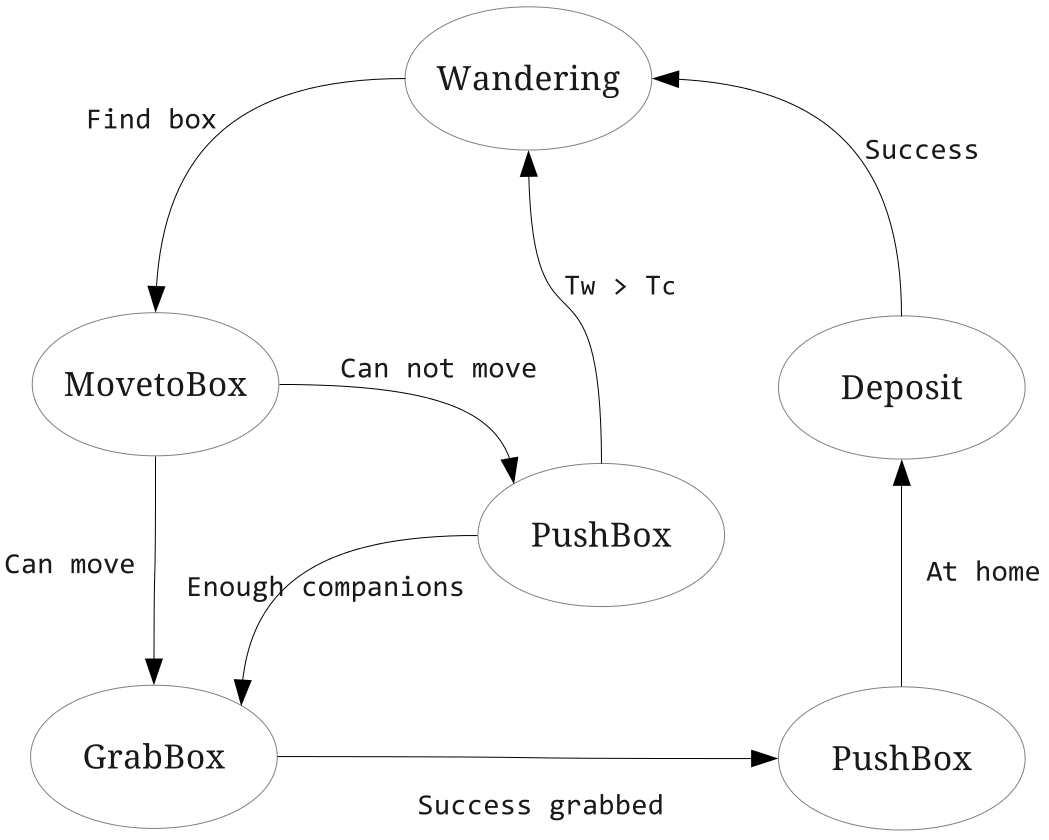
\includegraphics[width=2.5in]{state_trans.png}
\caption{A state transition diagram of robot in the box-pushing task.}
\label{fig:1}
\end{figure}
% Note that IEEE typically puts floats only at the top, even when this
% results in a large percentage of a column being occupied by floats.

\subsection{Energy Threshold Values Definition}
\label{subsec:2}
The energy of a robot is dependent on the energy consumption status of its motor and sensors. The total energy capacity of a robot is a constant value when the battery is fully charged. When the robot searches the boxes randomly or pushes the boxes, its remaining energy level can be calculated as follows:
%
\begin{equation}
E_{cur} = E_{full} - E_{sen} - E_{mot} - E_{com},
\label{eq:01}
\end{equation}
%
where $E_{cur}$ is the current energy status of a robot, $E_{full}$ is the energy of the robot when fully charged, $E_{sen}$ is the energy consumed by sensors; $E_{mot}$ is the energy consumed by motors; $E_{com}$ is the energy cost by the computing tasks of the robot. All energy can be calculated using (\ref{eq:01}).

Two energy threshold values are introduced for the robots to adapt their activities. (1). $Th_{c}$ is used to recommend the robot to come into requesting help state whenever it can or can not move the box. That is, the robot shifts the energy consumed task---pushing box---to other robots which have enough energy, after gathering enough other robots to move the box, the robot's state transforms into wandering. But when there is no robot come to help, a timer is needed to tick the waiting time $T_{c}$. The robot cancels its waiting when waiting time is expired and then goes on searching for boxes. The robot is searching and broadcasting its found information from boxes in its iteration. (2). $Th_{e}$ is used to stop movement of robot when its energy exhausted. When this state occurs, the robot needs to recharge its energy or just to rest if the recharge station is not available. Robots may not push the box when most of the robots are almost energy exhausted, therefore each robot is associated with another timer. The timer ticks increase when the detected box has not been pushed home. When it ticks up to the threshold $T_{p}$, the robots clear its waiting timer and push the box cooperatively with each other. In conclusion, robots share their energy by sharing tasks, and a robot makes a decision on sharing its own energy to others. The following part will show how the sharing scheme works.

\subsection{Energy-based Sharing}
\label{subsec:3}
The box-pushing mission includes three tasks: searching, calling for help and pushing the boxes home. Obviously, the pushing boxes and requesting help are the most and least energy consuming tasks, respectively. Based on this energy-consuming difference, each robot can switch itself to a more appropriate task according to its energy status.

\textbf{Searching phase.}The robot randomly search in the arena, if it receives a message indicating that a box is just detected by other robots, it will make a decision on helping according to its energy status. The decision is made by EPSO.

\textbf{Selecting phase.}When multi-boxes are identified by robots, each robot needs to decide the box it should push. All the robots may go to the same box and push it. This will lead to robots aggregated on one interested box, and fewer robots search the unknown boxes. To prevent this situation from occurring, a biologically inspired virtual pheromone trail mechanism is introduced. Each box is tagged with virtual pheromone density $\tau(t)$ that decreases with time. To emulate the increase and decrease procedures of pheromone trails in nature, the pheromone density maintained by robot $i$ is represented by:
%
\begin{equation}
\tau(t+1) = \rho\tau(t) + \Delta\tau_i,
\label{eq:02}
\end{equation}
%
where $\tau(t)$ is the pheromone density of the box before robot $i$ drops at time $t$, and $\Delta\tau_i$ is the pheromone robot $i$ dropped. $0<\rho<1$ is the pheromone decay parameter. Therefore at next iteration time $t+1$, the pheromone density of a box is $\tau(t+1)$.
If no robot updates the pheromone of the box, then the density will decay over time. However if the box is detected by some robots, the robots will update the pheromone periodically. The utility function of the box for a particular robot is defined as:
%
\begin{equation}
\mu(t) = \frac{\omega(t)}{d(t)}e^{-\tau(t)}e^{1-E_{con}/E_{cur}},
\label{eq:03}
\end{equation}
%
where $\omega(t)$ is the weight of the box defined as the number of robots required to move the box. $d(t)$ is the distance between robot $k$ and the box, and $e^{-\tau(t)}$ is the impact of the pheromone density associated with the box, $\tau(t)$ is the pheromone density defined in ~\ref{eq:02}; $e^{1-E_{con}/E_{cur}}$ is the energy factor for the robot, and $E_{cur}$ is current energy status of the robot, $E_{con}$ is the energy needed for the robot to push the box home.

The introduction of energy factor leads to a trade-off between task and energy. If the energy of a robot is insufficient for pushing a box, the attractiveness of the corresponding box will decreased. The robot needs to decide the particular box to push when multiple boxes are detected at a certain time. In this paper, the robot uses a Energy-based PSO algorithm to decide the particular box to help according to its internal status (energy status, waiting time) and social cues (number of neighbor robots and their energy status, etc.). The velocity vector of a particle in PSO is defined and updated as the followings:

\begin{equation}
\begin{split}
\mathbf{v}^{k}(t+1) &= \gamma_{e}\mathbf{v}^{k}(t) + \gamma_{c}rand_{c}(t)(p_{c}(t)-x^{k}(t)) +\\
&\gamma_{s}rand_{s}(t)(p_{s}(t)-x^{k}(t)),
\end{split}
\label{eq:04}
\end{equation}

where $\gamma_e$ represent the inertia weight, while $\gamma_c$ and $\gamma_s$ respectively represent the propensity constraint factors for cognitive and social behaviors. $0 \leq rand_c < 1$ and $0 \leq rand_s < 1$. $x^{k}(t)$ represents the position of agent $k$ at time $t$. $p_{s}(t)$ represents the global best from the neighbors, and $p_{c}(t)$ represents the local cognitive best. The position of particle can be updated as:
%
\begin{equation}
x^{k}(t+1) = x^{k}(t) + \mathbf{v}^{k}(t+1),
\label{eq:05}
\end{equation}

The swarm does not share any global information except the simulation map, thus the original PSO algorithm cannot be directly used. For example, it would be difficult to select global best. Therefore, the new velocity vector:
%
\begin{equation}
\mathbf{v}^{k}(t+1) = \gamma_{e}\mathbf{v}^{k}(t)\frac{\sum^n_{i=1}E_i}{nE_{cur}} + \gamma_{n}rand_{n}(t)(p_{n}(t)-x^{k}(t)),
\label{eq:06}
\end{equation}
%
where $\gamma_n$ represents the propensity constraint factors for local cognitive. $\sum^n_{i=1}E_i$ is the sum of the energy of the robots in the vicinity. $p_n(t)=max(\mu(t))$ is the local cognitive best position for the boxes detected by a robot.
The local cognitive best suggests that the appropriate robot push the most interested box to home while other robots searching for other boxes or communicating. Therefore, the robot with a higher energy level is tend to push the boxes and the robot with a lower energy level is more likely to communicate with neighbors, those actions are decided by EPSO.

\section{Scenario for Simulation}
\label{sec:3}
To validate the algorithm, the proposed algorithm is tested on the sensor-based simulation tools Player/Stage~\cite{Gerkey}. Player is a server that connects robots, sensors, and controls programs over a network. Stage simulates a population of mobile robots, sensors and objects in a two-dimensional bit-mapped environment. The simulation area is a 12.9m$\times$8.9m arena. Ten blocks are distributed randomly with different weight. Five homogeneous robots are used. The weight a box is not the same: some boxes only need one robot to push and others may need multiple ones. As in Fig.~\ref{fig:2}, the square at the right corner of the figure is home. The robot is equipped with two laser sensors, one camera named blob finder, one wifi, and one gripper, marked as red in simulation. Thus the robot can sense the box at a certain distance using the camera and can grab the detected box with its gripper. Moreover, it can use the laser sensors to avoid obstacles. Each robot knows how many boxes are placed in the arena, but does not know their position. Robots are placed in a arena, where they need to find the scattered boxes and push the found boxes home. Fig.~\ref{fig:3} is a snapshot of the robots. The mission is completed when one robot detects that all boxes are pushed home. Moreover, they should maintain their energy status to maintain a longer life.

% For figures use
%
\begin{figure}[h]
\begin{minipage}[t]{0.45\linewidth}
% Use the relevant command for your figure-insertion program
% to insert the figure file.
% For example, with the graphicx style use
\centering
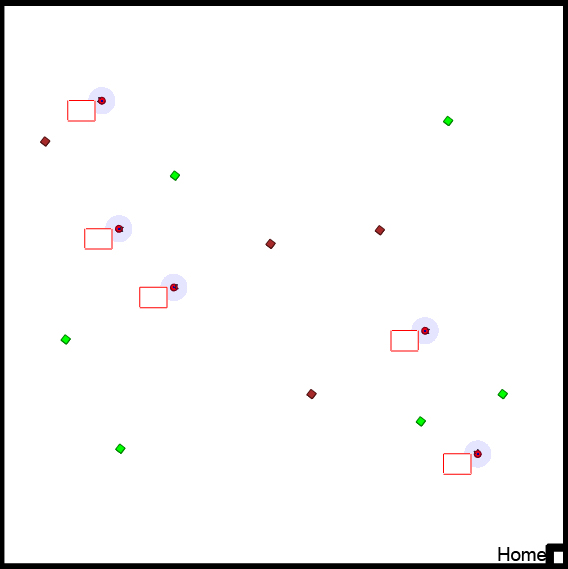
\includegraphics[width=1.6in]{scenario.png}
\caption{Screen shot of simulation. Five robots are equipped with two sick lasers, one camera and one gripper. The right corner of the screen is home.}
\label{fig:2}       % Give a unique label
\end{minipage}
\hfill
\begin{minipage}[t]{0.45\linewidth}
\centering
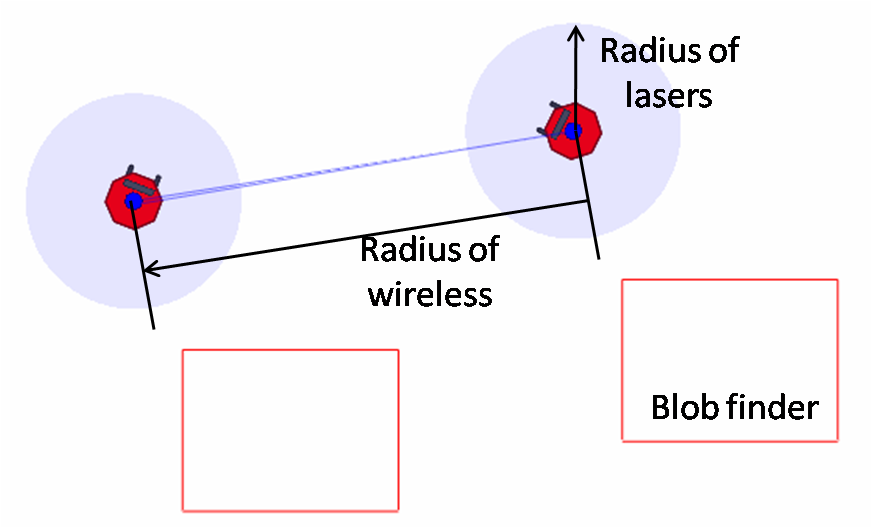
\includegraphics[width=1.6in]{robot.png}
\caption{Robot with laser range 1.0m, blob finder view distance is 2.0m, and wireless at range 5.0m.}
\label{fig:3}       % Give a unique label
\end{minipage}
\end{figure}

% An example of a double column floating figure using two subfigures.
% (The subfig.sty package must be loaded for this to work.)
% The subfigure \label commands are set within each subfloat command, the
% \label for the overall figure must come after \caption.
% \hfil must be used as a separator to get equal spacing.
% The subfigure.sty package works much the same way, except \subfigure is
% used instead of \subfloat.
%
%\begin{figure*}[!t]
%\centerline{\subfloat[Case I]\includegraphics[width=2.5in]{subfigcase1}%
%\label{fig_first_case}}
%\hfil
%\subfloat[Case II]{\includegraphics[width=2.5in]{subfigcase2}%
%\label{fig_second_case}}}
%\caption{Simulation results}
%\label{fig_sim}
%\end{figure*}
%
% Note that often IEEE papers with subfigures do not employ subfigure
% captions (using the optional argument to \subfloat), but instead will
% reference/describe all of them (a), (b), etc., within the main caption.


% An example of a floating table. Note that, for IEEE style tables, the 
% \caption command should come BEFORE the table. Table text will default to
% \footnotesize as IEEE normally uses this smaller font for tables.
% The \label must come after \caption as always.
%
%\begin{table}[!t]
%% increase table row spacing, adjust to taste
%\renewcommand{\arraystretch}{1.3}
% if using array.sty, it might be a good idea to tweak the value of
% \extrarowheight as needed to properly center the text within the cells
%\caption{An Example of a Table}
%\label{table_example}
%\centering
%% Some packages, such as MDW tools, offer better commands for making tables
%% than the plain LaTeX2e tabular which is used here.
%\begin{tabular}{|c||c|}
%\hline
%One & Two\\
%\hline
%Three & Four\\
%\hline
%\end{tabular}
%\end{table}


% Note that IEEE does not put floats in the very first column - or typically
% anywhere on the first page for that matter. Also, in-text middle ("here")
% positioning is not used. Most IEEE journals use top floats exclusively.
% Note that, LaTeX2e, unlike IEEE journals, places footnotes above bottom
% floats. This can be corrected via the \fnbelowfloat command of the
% stfloats package.

A simple energy consume model introduced by~\cite{Mei} is used to calculate the energy cost by each equipment of the robot. In the model, a linear function is posted for the energy consumption of the sensor:
%
\begin{equation}
p_s(f_s) = c_{s_0} + c_{s_1}(f_s),
\label{eq:07}
\end{equation}
%
where $f_s$ is the sensing frequencies, $p_s$ is the sensing power, $c_{s_0}$ and $c_{s_1}$ are two positive constant coefficients. Besides sensors power, motion power $p_m$ is proportional to the speed of the robot $v$ at different scenarios. In the experiments, the robot with 9kg load gets the linear function:

\begin{equation}
p_m(v) = 0.19 + 13.1v,
\label{eq:08}
\end{equation}
%
while the robot with no load has the linear function:
%
\begin{equation}
p_m(v) = 0.29 + 7.4v,
\label{eq:09}
\end{equation}

In the simulations, the energy consumption of a robot is calculated by equation (\ref{eq:09}) with no load, otherwise, the consumption function is switched to (\ref{eq:08}). The current energy level of a robot is recorded and its energy consumption is calculated as the input for EPSO algorithm.

\section{Experimental Results}
\label{sec:4}
\subsection{Selection of Parameters}
\label{subsec:1}
All robots are initially in the state of searching for the boxes. Each time a robot consumes a different amount of energy since the robot uses different sensors and actuators in different tasks. For example, compared to the action of wandering in the search area, a robot consumes more energy when carrying box back home because the gripper is used in the former state. Each sensor and actuator has a predefined value which represents the energy consumed by the component, and then these values are summed in accordance with the specific sensors and actuators used in the task. Table~\ref{tab:1} shows the energy consumed for each type of sensor each time used.
%%%%%%%%%%%%%%%%%%%%%%%%%%%%%%%%%%%%%%%%

\begin{table}[!t]
%% increase table row spacing, adjust to taste
\renewcommand{\arraystretch}{1.3}
% if using array.sty, it might be a good idea to tweak the value of
% \extrarowheight as needed to properly center the text within the cells
\caption{Energy consumed frequency for each sensor of a robot.}
\label{tab:1}
\centering
%% Some packages, such as MDW tools, offer better commands for making tables
%% than the plain LaTeX2e tabular which is used here.
\begin{tabular}{|c||c|}
\hline
Sensor & Energy consumed frequency\\
\hline
Laser & 0.02\\
\hline
Blob finder & 0.09\\
\hline
Wireless & 0.01\\
\hline
\end{tabular}
\end{table}

The parameters in Equation~\ref{eq:06} have been tested to get an optimal result. Table~\ref{tab:2} summarizes all of these parameters.
%%%%%%%%%%%%%%%%%%%%%%%%%%%%%%%%%%%%%%%%
\begin{table}[!t]
\renewcommand{\arraystretch}{1.3}
\caption{Parameters of EPSO}
\label{tab:2}
\centering
\begin{tabular}{|c||c||c||c||c|}
\hline
$Th_c$ & $Th_s$ & $\gamma_e$ & $\gamma_n$ & $E_{full}$ \\
\hline
0.2 & 0.08 & 0.9 & 0.1 & 1000000 \\
\hline
\end{tabular}
\end{table}
%
And $T_c$, the threshold of waiting time, is set to 200(iteration), here,  ``iteration'' is one iteration of PSO. 
\subsection{Simulation Results}
\label{subsec:2}
\textbf{Viability:} The EPSO algorithm is compared with the MS-PSO algorithm proposed by~\cite{Meng} which does not take energy shifting scheme into account. Firstly, the initialized energy is the same for the two methods; the remaining energy of each robot is recorded after the mission completed. In the experiment, the parameters and the initial battery energy for both algorithms are set to be the same, and the total energy capacity is 1000000J (joule). In order to reach a stable state, 20 respective tests are conducted to record remaining energy value of each robot. And the average of results from all the 20 tests is obtained. This group of experiment is repeated and the results are as Fig.~\ref{fig:4} a).
%
\begin{figure}[h]
\begin{center}
%\sidecaption
% Use the relevant command for your figure-insertion program
% to insert the figure file.
% For example, with the graphicx style use
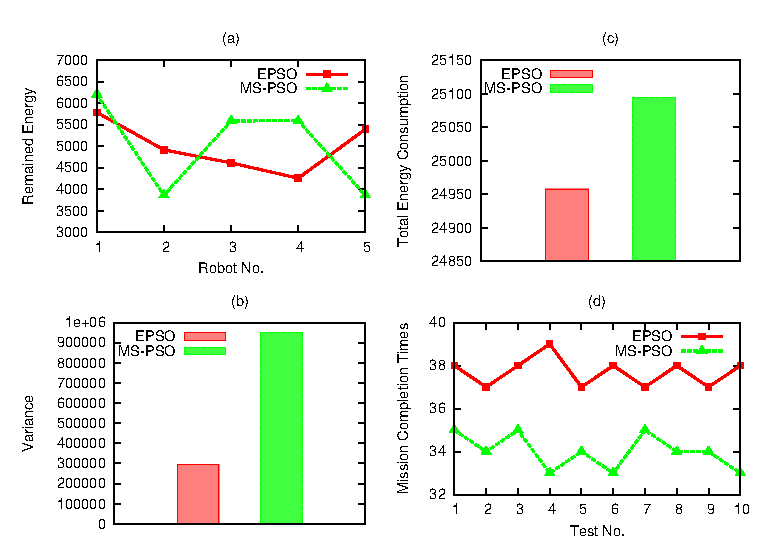
\includegraphics[scale=0.72]{result.eps}
%
% If no graphics program available, insert a blank space i.e. use
%\picplace{5cm}{2cm} % Give the correct figure height and width in cm
%
\caption{a) The remaining energy of the five robots after completing the box-pushing mission. b) Comparison of EPSO and the MS-PSO on variance. c) Comparison of the two methods on total energy consumption. d) Times of completed mission of the two methods.}
\label{fig:4}       % Give a unique label
\end{center}
\end{figure}
According to the results, the EPSO algorithm gets a more smooth line compared with the MS-PSO algorithm. This suggests that the EPSO algorithm has the ability to maintain the energy homeostasis for swarm of robots.

Furthermore, the variance of the results is calculated based on numbers of population. The fluctuation of the energy status of the robots is shown in Fig.~\ref{fig:4} b).

Compared to MS-PSO, the EPSO algorithm can improve the energy homeostasis of the swarm by 48.7\% on variance.

Fig.~\ref{fig:4} c) shows the total energy consumed by the swarm robots. The result indicates that the EPSO method reaches the same level of energy consumption as MS-PSO, but, as Fig.~\ref{fig:4} a) and Fig.~\ref{fig:4} b) show, with the same energy consumption, it makes a balanced energy distribution among the robots, thus reaches a more robust swarm. \\
\noindent\textbf{Effectiveness:} In this set of experiment, all the robots are fully charged in the beginning. When they complete one mission, they repeat the mission but maintain the current energy level instead of getting fulfilled again. The times the swarm completes the mission under certain total energy is recorded. And comparing EPSO with the MS-PSO, the result is shown in Fig.~\ref{fig:4} d).

The result indicates that the EPSO algorithm completes 3 or more missions than the MS-PSO on average. Therefore, initiated with the same amount of energy, the EPSO algorithm is able to make more efficient use of the battery energy.

\section{Conclusion}
\label{sec:5}
A novel energy-based task shifting algorithm EPSO for maintaining energy homeostasis of social autonomous swarm robots is proposed. Instead of transferring energy to the neighbors through hardware, EPSO shifts the task among neighbors. And the robot decides the initiation of shifting the task to other robots based on local information and its own energy status. Experimental results show that the proposed method is of better performance and suggest this approach is viable to reach energy homeostasis in social robots.
In the future, a self-sufficiency charging station will be built to supply the external energy for the social robots. And EPSO algorithm will be implemented and tested on the real robots.

% if have a single appendix:
%\appendix[Proof of the Zonklar Equations]
% or
%\appendix  % for no appendix heading
% do not use \section anymore after \appendix, only \section*
% is possibly needed

% use appendices with more than one appendix
% then use \section to start each appendix
% you must declare a \section before using any
% \subsection or using \label (\appendices by itself
% starts a section numbered zero.)
%

\appendices
%\section{Proof of the First Zonklar Equation}
%Appendix one text goes here.

% you can choose not to have a title for an appendix
% if you want by leaving the argument blank
%\section{}
%Appendix two text goes here.

% use section* for acknowledgement
\section*{Acknowledgment}
%The authors would like to thank...
This work was partly supported by the National Natural Science Foundation of China under Grant 60970107, 60970108 and the Key Program for Basic Research of Shanghai under Grant 08JC1411800.

% Can use something like this to put references on a page
% by themselves when using endfloat and the captionsoff option.
\ifCLASSOPTIONcaptionsoff
  \newpage
\fi

% trigger a \newpage just before the given reference
% number - used to balance the columns on the last page
% adjust value as needed - may need to be readjusted if
% the document is modified later
%\IEEEtriggeratref{8}
% The "triggered" command can be changed if desired:
%\IEEEtriggercmd{\enlargethispage{-5in}}

% references section

% can use a bibliography generated by BibTeX as a .bbl file
% BibTeX documentation can be easily obtained at:
% http://www.ctan.org/tex-archive/biblio/bibtex/contrib/doc/
% The IEEEtran BibTeX style support page is at:
% http://www.michaelshell.org/tex/ieeetran/bibtex/
%\bibliographystyle{IEEEtran}
% argument is your BibTeX string definitions and bibliography database(s)
%\bibliography{IEEEabrv,../bib/paper}
%
% <OR> manually copy in the resultant .bbl file
% set second argument of \begin to the number of references
% (used to reserve space for the reference number labels box)
\begin{thebibliography}{1}
\bibitem{Drener} 
Drenner, A., Papanikolopoulos, N.: Docking station relocation for maximizing longevity of distributed robotic teams, in Proceedings of the IEEE International Conference on Robotics and Automation, Orlando, FL, USA, pp. 2436--2441 (2006)
\bibitem{Du}
Du, Z., Li, H., Gu, T.: A state of the art review on microbial fuel cells: a promising technology for wastewater treatment and bioenergy, Biotechnol Adv Vol. \textbf{25}. 464–482 (2007)
\bibitem{Encyclopedia}
Encyclopedia Britannica, Homeostasis (2011) Encyclopedia Britannica Online: http://www.britannica.com/EBchecked/topic/270188/homeostasis
\bibitem{Gerkey}
Gerkey, B. P., Vaughan, R. T., Howard, A.: The player/stage project: tools for multi-robot and distributed sensor systems. In Proceedings of the International Conference on Advanced Robotics, Coimbra, Portugal. pp. 317--323 (2003)
\bibitem{Humza}
Humza, R., Scholz, O., Mokhtar, M., Timmis, J., Tyrrell, A.: Towards Energy Homeostasis in an Autonomous Self-Reconfigurable Modular Robotic Organism. In: Proc. of the First International Conference on Adaptive and Self-adaptive Systems and Applications, Comptation world, pp. 21--26. (2009)
\bibitem{Jones}
Jones, C. and Matari\'c, M.: Adaptive division of labor in large-scale minimalist multi-robot systems. In IEEE/RSJ International Conference on Intelligent Robots and Systems. pp. 1969--1974 (2003)
\bibitem{Kennedy}
Kennedy and R. Eberhart: Particle Swarm Optimization, IEEE onference on Neural Networks Proceedings. pp.1942--1948 (1995)
\bibitem{Krieger}
Krieger MJB, Billeter JB: The call of duty: Self-organised task allocation in a population of up to twelve mobile robots, Robotics and Autonomous Systems Vol. \textbf{30}, 65--84, Elsevier Science (2000)
\bibitem{Mataric}
Mataric J., Nilsson M., Simsarian K. T.: Cooperative Multi-robot Box-Pushing, IEEE/RSJ International Conference on Intelligent Robots and Systems, pp. 556--561 (1995)
\bibitem{McFarland}
McFarland, D., Spier E.: Basic Cycles, Utility and Opportunism in Self-Sufficient Robots, Robotics and Autonomous Systems, Vol. \textbf{20}, 179--190 (1997)
\bibitem{Mei}
Mei Y., Lu Y.-H., Hu Y. C., Lee C. G.: A Case Study of Mobile Robot's Energy Consumption and Conservation Techniques. In ICAR, pp. 492--497, (2005)
\bibitem{MelhuishK}
Melhuish, C., Kubo, M.: Collective Energy Distribution: Maintaining the Energy Balance in Distributed Autonomous Robots using Trophallaxis. In: Distributed Autonomous Robotic Systems 6, pp. 275--284. Springer, Heidelberg (2007)
\bibitem{MelhuishI}
Melhuish, C., Ieropoulos I., and  Greenman I., Horsfield, J.: Energetically autonomous robots: food for thought, Auton Robot, pp. 187--198 (2006)
\bibitem{Meng}
Meng, Y., Gan, J.: A Distributed Swarm Intelligence based Algorithm for a Cooperative Multi-Robot Construction Task. In: IEEE Swarm Intelligence Symposium, pp. 21--23 (2008)
\bibitem{Mokhtar}
Mokhtar M., Timmis J., Tyrrell A., Bi R.: An Artificial Lymph Node Architecture for Homeostasis in Collective Robotic Systems. In Workshop on Pervasive Adaptive Systems, Self-Adaptive and Self-Organizing Systems (SASO), Venice, Italy, pp. 126--131 (2008)
\bibitem{Ngo}
Ngo, T.D., Schi\o ler, H.: Sociable Robots through Self-maintained Energy. International Journal of Advanced Robotic Systems Vol. \textbf{3}, No. \textbf{4}. 313--322 (2006)
\bibitem{O'Hara}
O'Hara K., Nathuji R., Raj H., Schwan K., Balch T.: Autopower: Toward energy-aware software systems for distributed mobile robots. In IEEE International Conference on Robotics and Automation (ICRA), pp. 2757-2762 (2006)
\bibitem{Silverman}
Silverman M. C., Nies D., Jung B., Sukatme G. S.: Staying alive: A docking station for autonomous robot recharging, in Proceedings of the IEEE International Conference on Robotics and Automation, Washington, DC, pp. 1050--1055, (2002)
\bibitem{Walter}
Walter W. G.: The Living Brain. New York: W.W. Norton, 311 pp. (1953)
\end{thebibliography}

% biography section
% 
% If you have an EPS/PDF photo (graphicx package needed) extra braces are
% needed around the contents of the optional argument to biography to prevent
% the LaTeX parser from getting confused when it sees the complicated
% \includegraphics command within an optional argument. (You could create
% your own custom macro containing the \includegraphics command to make things
% simpler here.)
%\begin{biography}[{\includegraphics[width=1in,height=1.25in,clip,keepaspectratio]{mshell}}]{Michael Shell}
% or if you just want to reserve a space for a photo:

\begin{IEEEbiography}[{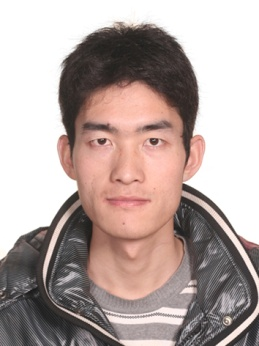
\includegraphics[width=1in,height=1.25in,clip,keepaspectratio]{zhouxin.jpg}}]{Xin Zhou}
is a graduate student in Shanghai Jiao Tong University. His research interests are Swarm Intelligence, Multi-agent Systems and Wireless Sensor Network. In MASS09 held in Macau, he received "Outstanding Demo. Award". He is applying the Ph.D. degree now.
\end{IEEEbiography}

% if you will not have a photo at all:
\begin{IEEEbiographynophoto}{Kai Xiao}
Biography text here.
\end{IEEEbiographynophoto}

% insert where needed to balance the two columns on the last page with
% biographies
%\newpage

\begin{IEEEbiographynophoto}{Yongfeng Xia}
is a master candidate in School of Software, Shanghai Jiao Tong University. His research interests are Swarm Intelligence, Swarm Robotics.
\end{IEEEbiographynophoto}

% You can push biographies down or up by placing
% a \vfill before or after them. The appropriate
% use of \vfill depends on what kind of text is
% on the last page and whether or not the columns
% are being equalized.

%\vfill

% Can be used to pull up biographies so that the bottom of the last one
% is flush with the other column.
%\enlargethispage{-5in}

% that's all folks
\end{document}


